
%(BEGIN_QUESTION)
% Copyright 2007, Tony R. Kuphaldt, released under the Creative Commons Attribution License (v 1.0)
% This means you may do almost anything with this work of mine, so long as you give me proper credit

The following control scheme adjusts wastewater flow though three clarifiers in a {\it sequenced} order:

$$\includegraphics[width=15.5cm]{i01808x01.eps}$$

Explain the operating philosophy of this control system.  Hint: the flow controllers are {\it direct acting} (i.e. they each open up their respective butterfly valve as the flow transmitter indicates a greater water flow rate).  Another hint: the total influent flow is not affected by the opening of the clarifier control valves.  Rather, the total influent flow is a function of water usage upstream of the wastewater clarifiers.

\vskip 20pt \vbox{\hrule \hbox{\strut \vrule{} {\bf Suggestions for Socratic discussion} \vrule} \hrule}

\begin{itemize}
\item{} A useful problem-solving strategy here is to add some numerical values to the diagram: assume a flow setpoint that is {\it less} than the total influent flow rate, then perform a ``thought experiment'' to see how the controllers would react to this.
\end{itemize}

\underbar{file i01808}
%(END_QUESTION)





%(BEGIN_ANSWER)

This control scheme tries to minimize the water flow rate through one clarifier while running the other clarifier(s) at a maximum flow rate value set by the HIC.

\vskip 10pt

The secret to understanding how this scheme works is to realize the total influent flow rate is fixed (coming from customers sending wastewater to be treated).  Opening up any one valve ``steals away'' water from the other clarifiers, such that each valve has an influence over {\it all} clarifier flow rates!

%(END_ANSWER)





%(BEGIN_NOTES)


%INDEX% Control, strategies: water clarifier sequenced flow control
%INDEX% Process: municipal water clarification

%(END_NOTES)


